\documentclass[twoside]{book}

% Packages required by doxygen
\usepackage{fixltx2e}
\usepackage{calc}
\usepackage{doxygen}
\usepackage[export]{adjustbox} % also loads graphicx
\usepackage{graphicx}
\usepackage[utf8]{inputenc}
\usepackage{makeidx}
\usepackage{multicol}
\usepackage{multirow}
\PassOptionsToPackage{warn}{textcomp}
\usepackage{textcomp}
\usepackage[nointegrals]{wasysym}
\usepackage[table]{xcolor}

% Font selection
\usepackage[T1]{fontenc}
\usepackage[scaled=.90]{helvet}
\usepackage{courier}
\usepackage{amssymb}
\usepackage{sectsty}
\renewcommand{\familydefault}{\sfdefault}
\allsectionsfont{%
  \fontseries{bc}\selectfont%
  \color{darkgray}%
}
\renewcommand{\DoxyLabelFont}{%
  \fontseries{bc}\selectfont%
  \color{darkgray}%
}
\newcommand{\+}{\discretionary{\mbox{\scriptsize$\hookleftarrow$}}{}{}}

% Page & text layout
\usepackage{geometry}
\geometry{%
  a4paper,%
  top=2.5cm,%
  bottom=2.5cm,%
  left=2.5cm,%
  right=2.5cm%
}
\tolerance=750
\hfuzz=15pt
\hbadness=750
\setlength{\emergencystretch}{15pt}
\setlength{\parindent}{0cm}
\setlength{\parskip}{3ex plus 2ex minus 2ex}
\makeatletter
\renewcommand{\paragraph}{%
  \@startsection{paragraph}{4}{0ex}{-1.0ex}{1.0ex}{%
    \normalfont\normalsize\bfseries\SS@parafont%
  }%
}
\renewcommand{\subparagraph}{%
  \@startsection{subparagraph}{5}{0ex}{-1.0ex}{1.0ex}{%
    \normalfont\normalsize\bfseries\SS@subparafont%
  }%
}
\makeatother

% Headers & footers
\usepackage{fancyhdr}
\pagestyle{fancyplain}
\fancyhead[LE]{\fancyplain{}{\bfseries\thepage}}
\fancyhead[CE]{\fancyplain{}{}}
\fancyhead[RE]{\fancyplain{}{\bfseries\leftmark}}
\fancyhead[LO]{\fancyplain{}{\bfseries\rightmark}}
\fancyhead[CO]{\fancyplain{}{}}
\fancyhead[RO]{\fancyplain{}{\bfseries\thepage}}
\fancyfoot[LE]{\fancyplain{}{}}
\fancyfoot[CE]{\fancyplain{}{}}
\fancyfoot[RE]{\fancyplain{}{\bfseries\scriptsize Generated by Doxygen }}
\fancyfoot[LO]{\fancyplain{}{\bfseries\scriptsize Generated by Doxygen }}
\fancyfoot[CO]{\fancyplain{}{}}
\fancyfoot[RO]{\fancyplain{}{}}
\renewcommand{\footrulewidth}{0.4pt}
\renewcommand{\chaptermark}[1]{%
  \markboth{#1}{}%
}
\renewcommand{\sectionmark}[1]{%
  \markright{\thesection\ #1}%
}

% Indices & bibliography
\usepackage{natbib}
\usepackage[titles]{tocloft}
\setcounter{tocdepth}{3}
\setcounter{secnumdepth}{5}
\makeindex

% Hyperlinks (required, but should be loaded last)
\usepackage{ifpdf}
\ifpdf
  \usepackage[pdftex,pagebackref=true]{hyperref}
\else
  \usepackage[ps2pdf,pagebackref=true]{hyperref}
\fi
\hypersetup{%
  colorlinks=true,%
  linkcolor=blue,%
  citecolor=blue,%
  unicode%
}

% Custom commands
\newcommand{\clearemptydoublepage}{%
  \newpage{\pagestyle{empty}\cleardoublepage}%
}

\usepackage{caption}
\captionsetup{labelsep=space,justification=centering,font={bf},singlelinecheck=off,skip=4pt,position=top}

%===== C O N T E N T S =====

\begin{document}

% Titlepage & ToC
\hypersetup{pageanchor=false,
             bookmarksnumbered=true,
             pdfencoding=unicode
            }
\pagenumbering{alph}
\begin{titlepage}
\vspace*{7cm}
\begin{center}%
{\Large Lab-\/3 }\\
\vspace*{1cm}
{\large Generated by Doxygen 1.8.13}\\
\end{center}
\end{titlepage}
\clearemptydoublepage
\pagenumbering{roman}
\tableofcontents
\clearemptydoublepage
\pagenumbering{arabic}
\hypersetup{pageanchor=true}

%--- Begin generated contents ---
\chapter{Московский государственный технический университет имени Н.\+Э. Баумана}
\label{md__r_e_a_d_m_e}
\Hypertarget{md__r_e_a_d_m_e}
\subsection*{Лабораторная работа по дисциплине БКИТ №X}

Выполнил\+: \href{https://vk.com/snipghost}{\tt Михаил Кучеренко \char`\"{}\+Snip\+Ghost\char`\"{}, ИУ5-\/34}, 18.\+10.\+2017 

~\newline


\subsubsection*{I. Описание задания}

Разработать программу, реализующую работу с классами.
\begin{DoxyEnumerate}
\item Программа должна быть разработана в виде консольного приложения на языке C\#.
\item Абстрактный класс «Геометрическая фигура» содержит виртуальный метод для вычисления площади фигуры.
\item Класс «Прямоугольник» наследуется от «Геометрическая фигура». Ширина и высота объявляются как свойства (property). Класс должен содержать конструктор по параметрам «ширина» и «высота».
\item Класс «Квадрат» наследуется от «Прямоугольник». Класс должен содержать конструктор по длине стороны.
\item Класс «Круг» наследуется от «Геометрическая фигура». Радиус объявляется как свойство (property). Класс должен содержать конструктор по параметру «радиус».
\item Для классов «Прямоугольник», «Квадрат», «Круг» переопределить виртуальный метод Object.\+To\+String(), который возвращает в виде строки основные параметры фигуры и ее площадь.
\item Разработать интерфейс I\+Print. Интерфейс содержит метод Print(), который не принимает параметров и возвращает void. Для классов «Прямоугольник», «Квадрат», «Круг» реализовать наследование от интерфейса I\+Print. Переопределяемый метод Print() выводит на консоль информацию, возвращаемую переопределенным методом To\+String(). 
\end{DoxyEnumerate}

~\newline


\subsubsection*{II. Код программы}


\begin{DoxyCode}
using System;
\textcolor{keyword}{using} System.Collections;
\textcolor{keyword}{using} System.Linq;
\textcolor{keyword}{using} System.Text;
\textcolor{keyword}{using} System.Threading.Tasks;

\textcolor{keyword}{namespace }\hyperlink{namespace_lab__3}{Lab\_3}
\{
    \textcolor{keyword}{class }Program
    \{

        \textcolor{keyword}{static} \textcolor{keywordtype}{void} Main()
        \{
            Menu m =\textcolor{keyword}{new} Menu();
            m.run();
        \}
    \}
\}
using System;

\textcolor{keyword}{namespace }\hyperlink{namespace_lab__3}{Lab\_3}
\{
    \textcolor{keyword}{interface }IPrint
    \{
        \textcolor{keywordtype}{void} print();
    \}
    \textcolor{keyword}{abstract} \textcolor{keyword}{class }Figure : IComparable, IPrint
    \{
        \textcolor{keyword}{virtual} \textcolor{keyword}{public} \textcolor{keywordtype}{double} square() \{ \textcolor{keywordflow}{return} 0; \}
        \textcolor{keyword}{public} \textcolor{keywordtype}{int} CompareTo(\textcolor{keywordtype}{object} obj)
        \{
            Figure f1 = obj as Figure;
            \textcolor{keywordflow}{if} (f1 == null)
                \textcolor{keywordflow}{throw} \textcolor{keyword}{new} ArgumentException(\textcolor{stringliteral}{"obj is not Figure!!!"});
            \textcolor{comment}{//if (this.square() > f1.square()) return 1;}
            \textcolor{comment}{//else if (this.square() == f1.square()) return 0;}
            \textcolor{comment}{//else return -1;}
            \textcolor{keywordflow}{return} this.square().CompareTo(f1.square());
        \}
        \textcolor{keyword}{abstract} \textcolor{keyword}{public} \textcolor{keywordtype}{void} print();

    \}
    \textcolor{keyword}{class }Circle : Figure
    \{
        \textcolor{keyword}{private} \textcolor{keywordtype}{double} r;
        \textcolor{keyword}{public} \textcolor{keywordtype}{double} radius
        \{
            \textcolor{keyword}{get}
            \{
                \textcolor{keywordflow}{return} r;
            \}
            \textcolor{keyword}{set}
            \{
                \textcolor{keywordflow}{if} (value < 0)
                    \textcolor{keywordflow}{throw} \textcolor{keyword}{new} ArgumentOutOfRangeException($\textcolor{stringliteral}{"\{nameof(value)\} должно быть положительным!"});
                r = value;
            \}
        \}
        \textcolor{keyword}{public} Circle(\textcolor{keywordtype}{double} r1)
        \{
            radius = r1;
        \}
        \textcolor{keyword}{public} \textcolor{keyword}{override} \textcolor{keywordtype}{string} ToString()
        \{
            \textcolor{keywordtype}{string} res;
            res = \textcolor{stringliteral}{"Class: Circle,"} +
               $\textcolor{stringliteral}{" Area: \{Math.Round(square(), 3)\}"};
            \textcolor{keywordflow}{return} res;
        \}
        \textcolor{keyword}{public} \textcolor{keyword}{override} \textcolor{keywordtype}{double} square()
        \{
            \textcolor{keywordflow}{return} Math.PI * r * r;
        \}
        \textcolor{keyword}{public} \textcolor{keyword}{override} \textcolor{keywordtype}{void} print()
        \{
            Console.WriteLine(this.ToString());
        \}

    \}
    \textcolor{keyword}{class }Rect : Figure
    \{
        \textcolor{keyword}{private} \textcolor{keywordtype}{double} a;
        \textcolor{keyword}{private} \textcolor{keywordtype}{double} b;
        \textcolor{keyword}{virtual} \textcolor{keyword}{public} \textcolor{keywordtype}{double} A
        \{
            \textcolor{keyword}{get}
            \{
                \textcolor{keywordflow}{return} a;
            \}
            \textcolor{keyword}{set}
            \{
                \textcolor{keywordflow}{if} (value < 0)
                    \textcolor{keywordflow}{throw} \textcolor{keyword}{new} ArgumentOutOfRangeException($\textcolor{stringliteral}{"\{nameof(value)\} должно быть положительным!"});
                a = value;
            \}
        \}
        \textcolor{keyword}{virtual} \textcolor{keyword}{public} \textcolor{keywordtype}{double} B
        \{
            \textcolor{keyword}{get}
            \{
                \textcolor{keywordflow}{return} b;
            \}
            \textcolor{keyword}{set}
            \{
                \textcolor{keywordflow}{if} (value < 0)
                    \textcolor{keywordflow}{throw} \textcolor{keyword}{new} ArgumentOutOfRangeException($\textcolor{stringliteral}{"\{nameof(value)\} должно быть положительным!"});
                b = value;
            \}
        \}
        \textcolor{keyword}{public} Rect(\textcolor{keywordtype}{double} a1, \textcolor{keywordtype}{double} b1)
        \{
            A = a1;
            B = b1;
        \}
        \textcolor{keyword}{public} \textcolor{keyword}{override} \textcolor{keywordtype}{string} ToString()
        \{
            \textcolor{keywordtype}{string} res;
            res = \textcolor{stringliteral}{"Class: Rectangle,"} +
               $\textcolor{stringliteral}{" Area: \{Math.Round(square(),3)\}"};
            \textcolor{keywordflow}{return} res;
        \}
        \textcolor{keyword}{public} \textcolor{keyword}{override} \textcolor{keywordtype}{double} square()
        \{
            \textcolor{keywordflow}{return} A * B;
        \}
        \textcolor{keyword}{public} \textcolor{keyword}{override} \textcolor{keywordtype}{void} print()
        \{
            Console.WriteLine(this.ToString());
        \}
    \}
    \textcolor{keyword}{class }Square : Rect
    \{
        \textcolor{keyword}{private} \textcolor{keywordtype}{double} a;
        \textcolor{comment}{//public override double A}
        \textcolor{comment}{//\{}
        \textcolor{comment}{//    get}
        \textcolor{comment}{//    \{}
        \textcolor{comment}{//        return a;}
        \textcolor{comment}{//    \}}
        \textcolor{comment}{//    set}
        \textcolor{comment}{//    \{}
        \textcolor{comment}{//        if (value < 0)}
        \textcolor{comment}{//            throw new ArgumentOutOfRangeException($"\{nameof(value)\} должно быть положительным!");}
        \textcolor{comment}{//        a = value;}
        \textcolor{comment}{//    \}}
        \textcolor{comment}{//\}}
        \textcolor{keyword}{public} \textcolor{keyword}{override} \textcolor{keywordtype}{string} ToString()
        \{
            \textcolor{keywordtype}{string} res;
            res = \textcolor{stringliteral}{"Class: Square,"} +
               $\textcolor{stringliteral}{" Area: \{Math.Round(square(), 3)\}"};
            \textcolor{keywordflow}{return} res;
        \}
        \textcolor{comment}{//public override double square()}
        \textcolor{comment}{//\{}
        \textcolor{comment}{//    return A * A;}
        \textcolor{comment}{//\}}
        \textcolor{keyword}{public} Square(\textcolor{keywordtype}{double} a1) : base(a1,a1)
        \{
        \}
    \}
\}
using System;
\textcolor{keyword}{using} System.Collections;
\textcolor{keyword}{using} System.Collections.Generic;
\textcolor{keyword}{using} System.Linq;
\textcolor{keyword}{using} System.Text;
\textcolor{keyword}{using} System.Threading.Tasks;

\textcolor{keyword}{namespace }\hyperlink{namespace_lab__3}{Lab\_3}
\{

    \textcolor{keyword}{class }TestArray : IPrint
    \{
        ArrayList arr1;
        Random rand;
        \textcolor{keyword}{public} TestArray()
        \{
            arr1 = \textcolor{keyword}{new} ArrayList();
            rand = \textcolor{keyword}{new} Random();
        \}
        \textcolor{keyword}{public} \textcolor{keywordtype}{void} Gener(\textcolor{keywordtype}{int} rmax, \textcolor{keywordtype}{int} times)
        \{
            \textcolor{keywordflow}{for} (\textcolor{keywordtype}{int} i = 0; i < times; i++)
            \{
                Figure res = null;
                \textcolor{keywordtype}{int} a = rand.Next(3);
                \textcolor{keywordflow}{switch} (a)
                \{
                    \textcolor{keywordflow}{case} 0:
                        res = \textcolor{keyword}{new} Circle(rand.Next(rmax));
                        \textcolor{keywordflow}{break};
                    \textcolor{keywordflow}{case} 1:
                        res = \textcolor{keyword}{new} Rect(rand.Next(rmax), rand.Next(rmax));
                        \textcolor{keywordflow}{break};
                    \textcolor{keywordflow}{case} 2:
                        res = \textcolor{keyword}{new} Square(rand.Next(rmax));
                        \textcolor{keywordflow}{break};
                \}
                arr1.Add(res);
            \}
        \}
        \textcolor{keyword}{public} \textcolor{keywordtype}{void} print()
        \{
            \textcolor{keywordflow}{foreach} (Figure f \textcolor{keywordflow}{in} arr1)
            \{
                f.print();
            \}
        \}
        \textcolor{keyword}{public} \textcolor{keywordtype}{void} Sort()
        \{
            arr1.Sort();
        \}
    \}
    \textcolor{comment}{//==================================}
    \textcolor{keyword}{public} \textcolor{keyword}{interface }IMatrAdapter<T>
    \{
       T getEmptyElement();
       \textcolor{keywordtype}{bool} checkEmptyElement(T element);
    \}
    \textcolor{keyword}{public} \textcolor{keyword}{class }FigureMatrixCheckEmpty : IMatrAdapter<Figure>
    \{
        Figure IMatrAdapter<Figure>.getEmptyElement()
        \{
            \textcolor{keywordflow}{return} null;
        \}
        \textcolor{keywordtype}{bool} IMatrAdapter<Figure>.checkEmptyElement(Figure element)
        \{
            \textcolor{keywordtype}{bool} res = \textcolor{keyword}{false};
            \textcolor{keywordflow}{if} (element == null)
                res = \textcolor{keyword}{true};
            \textcolor{keywordflow}{return} res;
        \}
    \}
    \textcolor{keyword}{class }Matrix<T>:IPrint
    \{
        \textcolor{keywordtype}{int} xmax, ymax, zmax;
        \textcolor{keyword}{public} IMatrAdapter<T> Adap;
        Dictionary<string, T> \_matr = \textcolor{keyword}{new} Dictionary<string, T>();
        \textcolor{keyword}{public} Matrix(\textcolor{keywordtype}{int} \_xmax, \textcolor{keywordtype}{int} \_ymax, \textcolor{keywordtype}{int} \_zmax, IMatrAdapter<T> IMCE)
        \{
            xmax = \_xmax;
            ymax = \_ymax;
            zmax = \_zmax;
            Adap = IMCE;
        \}
        \textcolor{keyword}{public} T \textcolor{keyword}{this}[\textcolor{keywordtype}{int} x, \textcolor{keywordtype}{int} y, \textcolor{keywordtype}{int} z]
        \{
            \textcolor{keyword}{set}
            \{
                CheckBounds(x, y, z);
                \textcolor{keywordtype}{string} key = DictKey(x, y, z);
                \textcolor{keywordflow}{if} (this.\_matr.ContainsKey(key))
                \{
                    this.\_matr[key] = value;
                \}
                \textcolor{keywordflow}{else}
                \{
                    this.\_matr.Add(key, value);
                \}
            \}
            \textcolor{keyword}{get}
            \{
                CheckBounds(x, y, z);
                \textcolor{keywordtype}{string} key = DictKey(x, y, z);
                \textcolor{keywordflow}{if} (this.\_matr.ContainsKey(key))
                \{
                    \textcolor{keywordflow}{return} this.\_matr[key];
                \}
                \textcolor{keywordflow}{else}
                \{
                    \textcolor{keywordflow}{return} this.Adap.getEmptyElement();
                \}
            \}
        \}
        \textcolor{keywordtype}{void} CheckBounds(\textcolor{keywordtype}{int} x, \textcolor{keywordtype}{int} y, \textcolor{keywordtype}{int} z)
        \{
            \textcolor{keywordflow}{if} (x < 0 || x >= xmax)
                \textcolor{keywordflow}{throw} \textcolor{keyword}{new} ArgumentOutOfRangeException(\textcolor{stringliteral}{"WRONG x"});
            \textcolor{keywordflow}{if} (y < 0 || y >= ymax)
                \textcolor{keywordflow}{throw} \textcolor{keyword}{new} ArgumentOutOfRangeException(\textcolor{stringliteral}{"WRONG y"});
            \textcolor{keywordflow}{if} (z < 0 || z >= zmax)
                \textcolor{keywordflow}{throw} \textcolor{keyword}{new} ArgumentOutOfRangeException(\textcolor{stringliteral}{"WRONG z"});

        \}
        \textcolor{keywordtype}{string} DictKey(\textcolor{keywordtype}{int} x, \textcolor{keywordtype}{int} y, \textcolor{keywordtype}{int} z)
        \{
            \textcolor{keywordflow}{return} x.ToString() + \textcolor{stringliteral}{"\_"} + y.ToString()+\textcolor{stringliteral}{"\_"}+ z.ToString();
        \}
        \textcolor{keyword}{public} \textcolor{keyword}{override} \textcolor{keywordtype}{string} ToString()
        \{
            StringBuilder res = \textcolor{keyword}{new} StringBuilder();
            res.Append(\textcolor{stringliteral}{"x | y | z | value\(\backslash\)n"});
            \textcolor{keywordflow}{for} (\textcolor{keywordtype}{int} i = 0; i < xmax; i++)
            \{
                \textcolor{keywordflow}{for} (\textcolor{keywordtype}{int} j = 0; j < ymax; j++)
                \{
                    \textcolor{keywordflow}{for} (\textcolor{keywordtype}{int} k = 0; k < zmax; k++)
                    \{
                        \textcolor{keywordflow}{if} (!Adap.checkEmptyElement(\textcolor{keyword}{this}[i, j, k]))
                        \{
                            res.Append(i.ToString()+\textcolor{stringliteral}{" | "}+j.ToString() + \textcolor{stringliteral}{" | "}+k.ToString() + \textcolor{stringliteral}{" | "}+\textcolor{keyword}{this}[i,
       j, k].ToString()+\textcolor{stringliteral}{"\(\backslash\)n"});
                        \}
                    \}
                \}
            \}
            res.Append(\textcolor{stringliteral}{"All other elements are empty\(\backslash\)n"});
            \textcolor{keywordflow}{return} res.ToString();
        \}
        \textcolor{keyword}{public} \textcolor{keywordtype}{void} print()
        \{
            Console.WriteLine(this.ToString());
        \}
    \}
    \textcolor{comment}{//==================================}
    \textcolor{keyword}{class }SimpleList<T> : IPrint
        where T : IComparable
    \{
        \textcolor{keyword}{protected} SimpleListItem<T> first;
        \textcolor{keyword}{protected} SimpleListItem<T> last;
        \textcolor{keywordtype}{int} \_count;
        \textcolor{keyword}{public} SimpleList()
        \{
            first = null;
            last = null;
        \}
        \textcolor{keyword}{public} \textcolor{keywordtype}{int} count
        \{
            \textcolor{keyword}{get}
            \{
                \textcolor{keywordflow}{return} \_count;
            \}
            \textcolor{keyword}{protected} \textcolor{keyword}{set}
            \{
                \_count = value;
            \}
        \}
        \textcolor{keyword}{public} \textcolor{keywordtype}{void} Add(T element)
        \{
            SimpleListItem<T> a = \textcolor{keyword}{new} SimpleListItem<T>(element);
            \textcolor{keywordflow}{if} (this.last == null)
            \{
                first = a;
                last = a;
            \}
            \textcolor{keywordflow}{else}
            \{
                last.next = a;
                last = a;
            \}
            count++;
        \}
        \textcolor{keyword}{public} SimpleListItem<T> getItem(\textcolor{keywordtype}{int} number)
        \{
            \textcolor{keywordflow}{if} (number < 0 || number >= count)
            \{
                \textcolor{keywordflow}{throw} \textcolor{keyword}{new} ArgumentException(\textcolor{stringliteral}{"WRONG INDEX"});
            \}
            \textcolor{keywordflow}{else}
            \{
                \textcolor{keywordtype}{int} i = 0;
                SimpleListItem<T> buf = this.first;
                \textcolor{keywordflow}{while} (i<number)
                \{
                    i++;
                    buf = buf.next;
                \}
                \textcolor{keywordflow}{return} buf;
            \}
        \}
        \textcolor{keyword}{public} T Get(\textcolor{keywordtype}{int} number)
        \{
            \textcolor{keywordflow}{return} getItem(number).data;
        \}
        \textcolor{keyword}{public} \textcolor{keyword}{override} \textcolor{keywordtype}{string} ToString()
        \{
            StringBuilder res = \textcolor{keyword}{new} StringBuilder();
            \textcolor{keywordflow}{for} (\textcolor{keywordtype}{int} i = 0; i < count; i++)
            \{
                res.Append(i.ToString()+\textcolor{stringliteral}{") "}+Get(i).ToString()+\textcolor{stringliteral}{"\(\backslash\)n"});
            \}
            \textcolor{keywordflow}{return} res.ToString();
        \}
        \textcolor{keyword}{public} \textcolor{keywordtype}{void} print()
        \{
            Console.WriteLine(this.ToString());
        \}
    \}
    \textcolor{keyword}{class }SimpleListItem<T>
        where T : IComparable
    \{
        \textcolor{keyword}{public} SimpleListItem(T param)
        \{
            data = param;
        \}
        \textcolor{keyword}{public} T data
        \{
            \textcolor{keyword}{get}
            \{
                \textcolor{keywordflow}{return} \_data;
            \}
            \textcolor{keyword}{set}
            \{
                \_data = value;
            \}
        \}
        T \_data;
        \textcolor{keyword}{public} SimpleListItem<T> next
        \{
            \textcolor{keyword}{get}
            \{
                \textcolor{keywordflow}{return} \_next;
            \}
            \textcolor{keyword}{set}
            \{
                \_next = value;
            \}
        \}
        SimpleListItem<T> \_next = null;
    \}
    \textcolor{keyword}{class }SimpleStack<T> : SimpleList<T>
        where T:IComparable
    \{
        \textcolor{keyword}{public} SimpleListItem<T> Pop(\textcolor{keywordtype}{int} i)
        \{
            SimpleListItem<T> buf = getItem(i);
            \textcolor{keywordflow}{if} (first == buf)
            \{
                first = buf.next;\textcolor{comment}{//ошибка, если в списке 1 элемент!}
                \textcolor{keywordflow}{if} (count == 1)
                    last = null;
            \}
            \textcolor{keywordflow}{else}
            \{
                getItem(i - 1).next = buf.next;
            \}
            count--;
            \textcolor{keywordflow}{return} buf;
        \}
        \textcolor{keyword}{public} \textcolor{keywordtype}{void} Push(T element)
        \{
            Add(element);
        \}
    \}
    \textcolor{comment}{//==================================}
    \textcolor{keyword}{class }Menu
    \{
        MySystem mySys = \textcolor{keyword}{new} MySystem();
        \textcolor{keywordtype}{int} intReadKey()
        \{
            \textcolor{keywordtype}{int} res;
            \textcolor{keywordtype}{bool} f = \textcolor{keywordtype}{int}.TryParse(Console.ReadLine(), out res);
            \textcolor{keywordflow}{if} (!f)
                \textcolor{keywordflow}{throw} \textcolor{keyword}{new} ArgumentException(\textcolor{stringliteral}{"Wrong input"});
            \textcolor{keywordflow}{return} res;
        \}
        \textcolor{keywordtype}{void} case1()
        \{
            Console.Clear();
            Console.Write(\textcolor{stringliteral}{"Enter number of elements. Array will be filled by randomly generated figures: "})
      ;
            TestArray a = \textcolor{keyword}{new} TestArray();
            a.Gener(10, intReadKey());
            mySys.printPalka(20);
            a.print();
            mySys.printPalka(20);
            Console.WriteLine(\textcolor{stringliteral}{"Sorting..."});
            mySys.printPalka(20);
            a.Sort();
            a.print();
        \}
        \textcolor{keywordtype}{void} case2()
        \{
            Console.Clear();
            Console.Write(\textcolor{stringliteral}{"Enter maximum size: "});
            \textcolor{keywordtype}{int} rmax= intReadKey();
            Console.Write(\textcolor{stringliteral}{"Enter number of elements generated: "});
            \textcolor{keywordtype}{int} times = intReadKey();
            mySys.printPalka(20);
            Random rand = \textcolor{keyword}{new} Random();
            Matrix<Figure> matr = \textcolor{keyword}{new} Matrix<Figure>(rmax,rmax,rmax,\textcolor{keyword}{new} FigureMatrixCheckEmpty());
            \textcolor{keywordflow}{for} (\textcolor{keywordtype}{int} i = 0; i < times; i++)
            \{
                \textcolor{keywordtype}{int} i0 = rand.Next(rmax), i1 = rand.Next(rmax), i2 = rand.Next(rmax);
                matr[i0, i1, i2] = mySys.GenerFigure(10, rand);
            \}
            Console.WriteLine(\textcolor{stringliteral}{"Printing existing elements..."});
            mySys.printPalka(20);
            matr.print();
        \}
        \textcolor{keywordtype}{void} case3()
        \{
            Console.Clear();
            Console.Write(\textcolor{stringliteral}{"Enter number of elements generated: "});
            \textcolor{keywordtype}{int} times = intReadKey();
            SimpleStack<Figure> a = \textcolor{keyword}{new} SimpleStack<Figure>();
            Random rand = \textcolor{keyword}{new} Random();
            \textcolor{keywordflow}{for} (\textcolor{keywordtype}{int} i = 0; i < times; i++)
            \{
                a.Push(mySys.GenerFigure(10, rand));
            \}
            Console.WriteLine(\textcolor{stringliteral}{"Printing generated data..."});
            mySys.printPalka(20);
            a.print();
            mySys.printPalka(20);
            Console.Write(\textcolor{stringliteral}{"Enter number of eliminating element: "});
            \textcolor{keywordtype}{bool} t = \textcolor{keyword}{true};
            SimpleListItem<Figure> f = null;
            \textcolor{keywordflow}{while} (t)
            \{
                times = intReadKey();
                \textcolor{keywordflow}{try}
                \{
                    f = a.Pop(times);
                    t = \textcolor{keyword}{false};
                \}
                \textcolor{keywordflow}{catch} (ArgumentException)
                \{
                    Console.Write(\textcolor{stringliteral}{"Wrong input! Please, enter again: "});
                    \textcolor{keywordflow}{continue};
                \}
            \}
            mySys.printPalka(20);
            Console.WriteLine(\textcolor{stringliteral}{"Eliminated element : "} + f.data.ToString());
            mySys.printPalka(20);
            Console.WriteLine(\textcolor{stringliteral}{"Printing stack: "});
            a.print();
        \}
        \textcolor{keyword}{public} \textcolor{keywordtype}{void} run()
        \{
            \textcolor{keywordtype}{bool} t = \textcolor{keyword}{true};
            \textcolor{keywordtype}{bool} p = \textcolor{keyword}{true};
            \textcolor{keywordflow}{while} (p)
            \{
                Console.Clear();
                \textcolor{keywordflow}{if} (t) Console.WriteLine(\textcolor{stringliteral}{"Lab\_3 by Baybarin R.\(\backslash\)n"});
                t = \textcolor{keyword}{false};
                Console.Write(\textcolor{stringliteral}{"============\(\backslash\)n"} +
                              \textcolor{stringliteral}{"Menu\(\backslash\)n"} +
                              \textcolor{stringliteral}{"============\(\backslash\)n"} +
                              \textcolor{stringliteral}{"1) Testing ArrayList.Sort()\(\backslash\)n"} +
                              \textcolor{stringliteral}{"2) Testing Sparse Matrix\(\backslash\)n"} +
                              \textcolor{stringliteral}{"3) Testing SimpleList\(\backslash\)n"} +
                              \textcolor{stringliteral}{"0) Exit\(\backslash\)n"} +
                              \textcolor{stringliteral}{"============\(\backslash\)n"} +
                              \textcolor{stringliteral}{"Your choice: "});
                \textcolor{keywordtype}{int} caseSwitch;
                \textcolor{keywordtype}{bool} f;
                f = \textcolor{keywordtype}{int}.TryParse(Console.ReadLine(), out caseSwitch);
                \textcolor{keywordflow}{if} (!f || caseSwitch < 0 || caseSwitch > 3)
                \{
                    Console.WriteLine(\textcolor{stringliteral}{"ERROR!!!!! WRONG INPUT"});
                    mySys.pause();
                    \textcolor{keywordflow}{continue};
                \}
                \textcolor{keywordflow}{switch} (caseSwitch)
                \{
                    \textcolor{keywordflow}{case} 0:
                        p = \textcolor{keyword}{false};
                        Console.WriteLine(\textcolor{stringliteral}{"Exiting...Press Enter"});
                        \textcolor{keywordflow}{break};
                    \textcolor{keywordflow}{case} 1: case1();
                        \textcolor{keywordflow}{break};
                    \textcolor{keywordflow}{case} 2: case2();
                        \textcolor{keywordflow}{break};
                    \textcolor{keywordflow}{case} 3: case3();
                        \textcolor{keywordflow}{break};
                \}
                mySys.pause();
            \}
        \}
    \}
\}
using System;
\textcolor{keyword}{using} System.Collections.Generic;
\textcolor{keyword}{using} System.Linq;
\textcolor{keyword}{using} System.Text;
\textcolor{keyword}{using} System.Threading.Tasks;

\textcolor{keyword}{namespace }\hyperlink{namespace_lab__3}{Lab\_3}
\{
    \textcolor{keyword}{class }MySystem
    \{
        \textcolor{keyword}{public} \textcolor{keywordtype}{void} pause()
        \{
            Console.WriteLine(\textcolor{stringliteral}{"Input enter..."});
            Console.ReadLine();
        \}
        \textcolor{keyword}{public} \textcolor{keywordtype}{void} printPalka(\textcolor{keywordtype}{int} l)
        \{
            \textcolor{keywordflow}{for} (\textcolor{keywordtype}{int} i = 0; i < l; i++)
            \{
                Console.Write(\textcolor{stringliteral}{"="});
            \}
            Console.Write(\textcolor{stringliteral}{"\(\backslash\)n"});
        \}
        \textcolor{keyword}{public} Figure GenerFigure(\textcolor{keywordtype}{int} param, Random rand)
        \{
            Figure res = null;
            \textcolor{keywordtype}{int} a = rand.Next(3);
            \textcolor{keywordflow}{switch} (a)
            \{
                \textcolor{keywordflow}{case} 0:
                    res = \textcolor{keyword}{new} Circle(rand.Next(param));
                    \textcolor{keywordflow}{break};
                \textcolor{keywordflow}{case} 1:
                    res = \textcolor{keyword}{new} Rect(rand.Next(param), rand.Next(param));
                    \textcolor{keywordflow}{break};
                \textcolor{keywordflow}{case} 2:
                    res = \textcolor{keyword}{new} Square(rand.Next(param));
                    \textcolor{keywordflow}{break};
            \}
            \textcolor{keywordflow}{return} res;
        \}
    \}
\}
\end{DoxyCode}


\href{Program.cs}{\tt Исходный код} 

~\newline


\subsubsection*{I\+II. Примеры работы}

~\newline

\chapter{Namespace Index}
\section{Packages}
Here are the packages with brief descriptions (if available)\+:\begin{DoxyCompactList}
\item\contentsline{section}{\hyperlink{namespace_lab__3}{Lab\+\_\+3} }{\pageref{namespace_lab__3}}{}
\end{DoxyCompactList}

\chapter{Hierarchical Index}
\section{Class Hierarchy}
This inheritance list is sorted roughly, but not completely, alphabetically\+:\begin{DoxyCompactList}
\item I\+Comparable\begin{DoxyCompactList}
\item \contentsline{section}{Lab\+\_\+3.\+Figure}{\pageref{class_lab__3_1_1_figure}}{}
\begin{DoxyCompactList}
\item \contentsline{section}{Lab\+\_\+3.\+Circle}{\pageref{class_lab__3_1_1_circle}}{}
\item \contentsline{section}{Lab\+\_\+3.\+Rect}{\pageref{class_lab__3_1_1_rect}}{}
\begin{DoxyCompactList}
\item \contentsline{section}{Lab\+\_\+3.\+Square}{\pageref{class_lab__3_1_1_square}}{}
\end{DoxyCompactList}
\end{DoxyCompactList}
\end{DoxyCompactList}
\item \contentsline{section}{Lab\+\_\+3.\+I\+Matr\+Adapter$<$ T $>$}{\pageref{interface_lab__3_1_1_i_matr_adapter}}{}
\item \contentsline{section}{Lab\+\_\+3.\+I\+Matr\+Adapter$<$ Figure $>$}{\pageref{interface_lab__3_1_1_i_matr_adapter}}{}
\begin{DoxyCompactList}
\item \contentsline{section}{Lab\+\_\+3.\+Figure\+Matrix\+Check\+Empty}{\pageref{class_lab__3_1_1_figure_matrix_check_empty}}{}
\end{DoxyCompactList}
\item \contentsline{section}{Lab\+\_\+3.\+I\+Print}{\pageref{interface_lab__3_1_1_i_print}}{}
\begin{DoxyCompactList}
\item \contentsline{section}{Lab\+\_\+3.\+Figure}{\pageref{class_lab__3_1_1_figure}}{}
\item \contentsline{section}{Lab\+\_\+3.\+Matrix$<$ T $>$}{\pageref{class_lab__3_1_1_matrix}}{}
\item \contentsline{section}{Lab\+\_\+3.\+Simple\+List$<$ T $>$}{\pageref{class_lab__3_1_1_simple_list}}{}
\begin{DoxyCompactList}
\item \contentsline{section}{Lab\+\_\+3.\+Simple\+Stack$<$ T $>$}{\pageref{class_lab__3_1_1_simple_stack}}{}
\end{DoxyCompactList}
\item \contentsline{section}{Lab\+\_\+3.\+Test\+Array}{\pageref{class_lab__3_1_1_test_array}}{}
\end{DoxyCompactList}
\item \contentsline{section}{Lab\+\_\+3.\+Menu}{\pageref{class_lab__3_1_1_menu}}{}
\item \contentsline{section}{Lab\+\_\+3.\+My\+System}{\pageref{class_lab__3_1_1_my_system}}{}
\item \contentsline{section}{Lab\+\_\+3.\+Program}{\pageref{class_lab__3_1_1_program}}{}
\item \contentsline{section}{Lab\+\_\+3.\+Simple\+List\+Item$<$ T $>$}{\pageref{class_lab__3_1_1_simple_list_item}}{}
\end{DoxyCompactList}

\chapter{Class Index}
\section{Class List}
Here are the classes, structs, unions and interfaces with brief descriptions\+:\begin{DoxyCompactList}
\item\contentsline{section}{\hyperlink{class_lab__3_1_1_circle}{Lab\+\_\+3.\+Circle} }{\pageref{class_lab__3_1_1_circle}}{}
\item\contentsline{section}{\hyperlink{class_lab__3_1_1_figure}{Lab\+\_\+3.\+Figure} }{\pageref{class_lab__3_1_1_figure}}{}
\item\contentsline{section}{\hyperlink{class_lab__3_1_1_figure_matrix_check_empty}{Lab\+\_\+3.\+Figure\+Matrix\+Check\+Empty} }{\pageref{class_lab__3_1_1_figure_matrix_check_empty}}{}
\item\contentsline{section}{\hyperlink{interface_lab__3_1_1_i_matr_adapter}{Lab\+\_\+3.\+I\+Matr\+Adapter$<$ T $>$} }{\pageref{interface_lab__3_1_1_i_matr_adapter}}{}
\item\contentsline{section}{\hyperlink{interface_lab__3_1_1_i_print}{Lab\+\_\+3.\+I\+Print} }{\pageref{interface_lab__3_1_1_i_print}}{}
\item\contentsline{section}{\hyperlink{class_lab__3_1_1_matrix}{Lab\+\_\+3.\+Matrix$<$ T $>$} }{\pageref{class_lab__3_1_1_matrix}}{}
\item\contentsline{section}{\hyperlink{class_lab__3_1_1_menu}{Lab\+\_\+3.\+Menu} }{\pageref{class_lab__3_1_1_menu}}{}
\item\contentsline{section}{\hyperlink{class_lab__3_1_1_my_system}{Lab\+\_\+3.\+My\+System} }{\pageref{class_lab__3_1_1_my_system}}{}
\item\contentsline{section}{\hyperlink{class_lab__3_1_1_program}{Lab\+\_\+3.\+Program} }{\pageref{class_lab__3_1_1_program}}{}
\item\contentsline{section}{\hyperlink{class_lab__3_1_1_rect}{Lab\+\_\+3.\+Rect} }{\pageref{class_lab__3_1_1_rect}}{}
\item\contentsline{section}{\hyperlink{class_lab__3_1_1_simple_list}{Lab\+\_\+3.\+Simple\+List$<$ T $>$} }{\pageref{class_lab__3_1_1_simple_list}}{}
\item\contentsline{section}{\hyperlink{class_lab__3_1_1_simple_list_item}{Lab\+\_\+3.\+Simple\+List\+Item$<$ T $>$} }{\pageref{class_lab__3_1_1_simple_list_item}}{}
\item\contentsline{section}{\hyperlink{class_lab__3_1_1_simple_stack}{Lab\+\_\+3.\+Simple\+Stack$<$ T $>$} }{\pageref{class_lab__3_1_1_simple_stack}}{}
\item\contentsline{section}{\hyperlink{class_lab__3_1_1_square}{Lab\+\_\+3.\+Square} }{\pageref{class_lab__3_1_1_square}}{}
\item\contentsline{section}{\hyperlink{class_lab__3_1_1_test_array}{Lab\+\_\+3.\+Test\+Array} }{\pageref{class_lab__3_1_1_test_array}}{}
\end{DoxyCompactList}

\chapter{Namespace Documentation}
\hypertarget{namespace_lab__3}{}\section{Lab\+\_\+3 Namespace Reference}
\label{namespace_lab__3}\index{Lab\+\_\+3@{Lab\+\_\+3}}
\subsection*{Classes}
\begin{DoxyCompactItemize}
\item 
class \hyperlink{class_lab__3_1_1_circle}{Circle}
\item 
class \hyperlink{class_lab__3_1_1_figure}{Figure}
\item 
class \hyperlink{class_lab__3_1_1_figure_matrix_check_empty}{Figure\+Matrix\+Check\+Empty}
\item 
interface \hyperlink{interface_lab__3_1_1_i_matr_adapter}{I\+Matr\+Adapter}
\item 
interface \hyperlink{interface_lab__3_1_1_i_print}{I\+Print}
\item 
class \hyperlink{class_lab__3_1_1_matrix}{Matrix}
\item 
class \hyperlink{class_lab__3_1_1_menu}{Menu}
\item 
class \hyperlink{class_lab__3_1_1_my_system}{My\+System}
\item 
class \hyperlink{class_lab__3_1_1_program}{Program}
\item 
class \hyperlink{class_lab__3_1_1_rect}{Rect}
\item 
class \hyperlink{class_lab__3_1_1_simple_list}{Simple\+List}
\item 
class \hyperlink{class_lab__3_1_1_simple_list_item}{Simple\+List\+Item}
\item 
class \hyperlink{class_lab__3_1_1_simple_stack}{Simple\+Stack}
\item 
class \hyperlink{class_lab__3_1_1_square}{Square}
\item 
class \hyperlink{class_lab__3_1_1_test_array}{Test\+Array}
\end{DoxyCompactItemize}

\chapter{Class Documentation}
\hypertarget{class_lab__3_1_1_circle}{}\section{Lab\+\_\+3.\+Circle Class Reference}
\label{class_lab__3_1_1_circle}\index{Lab\+\_\+3.\+Circle@{Lab\+\_\+3.\+Circle}}
Inheritance diagram for Lab\+\_\+3.\+Circle\+:\begin{figure}[H]
\begin{center}
\leavevmode
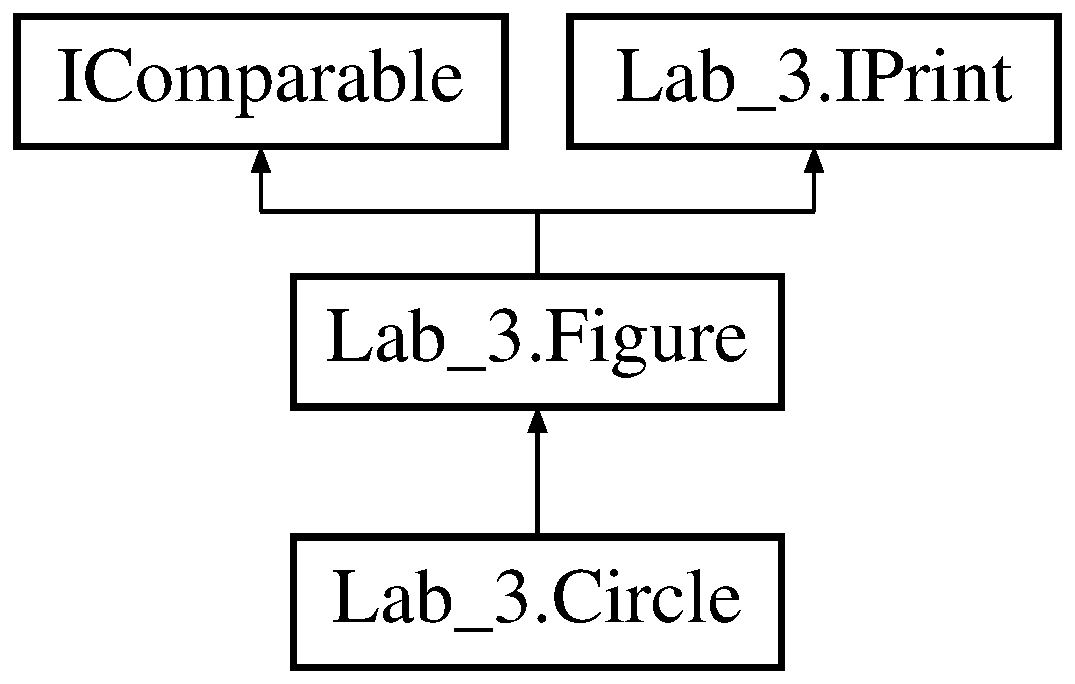
\includegraphics[height=3.000000cm]{class_lab__3_1_1_circle}
\end{center}
\end{figure}
\subsection*{Public Member Functions}
\begin{DoxyCompactItemize}
\item 
\mbox{\Hypertarget{class_lab__3_1_1_circle_a50b6f520152c103aee4d74ede90eb846}\label{class_lab__3_1_1_circle_a50b6f520152c103aee4d74ede90eb846}} 
{\bfseries Circle} (double r1)
\item 
\mbox{\Hypertarget{class_lab__3_1_1_circle_ab438980b622a5782df87857b535b83ad}\label{class_lab__3_1_1_circle_ab438980b622a5782df87857b535b83ad}} 
override string {\bfseries To\+String} ()
\item 
\mbox{\Hypertarget{class_lab__3_1_1_circle_a6ae76b7d2380174acc20b067a3322fa6}\label{class_lab__3_1_1_circle_a6ae76b7d2380174acc20b067a3322fa6}} 
override double {\bfseries square} ()
\item 
\mbox{\Hypertarget{class_lab__3_1_1_circle_abccde0979b32c677a4f936d1402e6e16}\label{class_lab__3_1_1_circle_abccde0979b32c677a4f936d1402e6e16}} 
override void {\bfseries print} ()
\end{DoxyCompactItemize}
\subsection*{Properties}
\begin{DoxyCompactItemize}
\item 
\mbox{\Hypertarget{class_lab__3_1_1_circle_a4ae0b6e9b619436762f35761a31816b8}\label{class_lab__3_1_1_circle_a4ae0b6e9b619436762f35761a31816b8}} 
double {\bfseries radius}\hspace{0.3cm}{\ttfamily  \mbox{[}get, set\mbox{]}}
\end{DoxyCompactItemize}


The documentation for this class was generated from the following file\+:\begin{DoxyCompactItemize}
\item 
Lab\+\_\+2\+\_\+\+Source.\+cs\end{DoxyCompactItemize}

\hypertarget{class_lab__3_1_1_figure}{}\section{Lab\+\_\+3.\+Figure Class Reference}
\label{class_lab__3_1_1_figure}\index{Lab\+\_\+3.\+Figure@{Lab\+\_\+3.\+Figure}}
Inheritance diagram for Lab\+\_\+3.\+Figure\+:\begin{figure}[H]
\begin{center}
\leavevmode
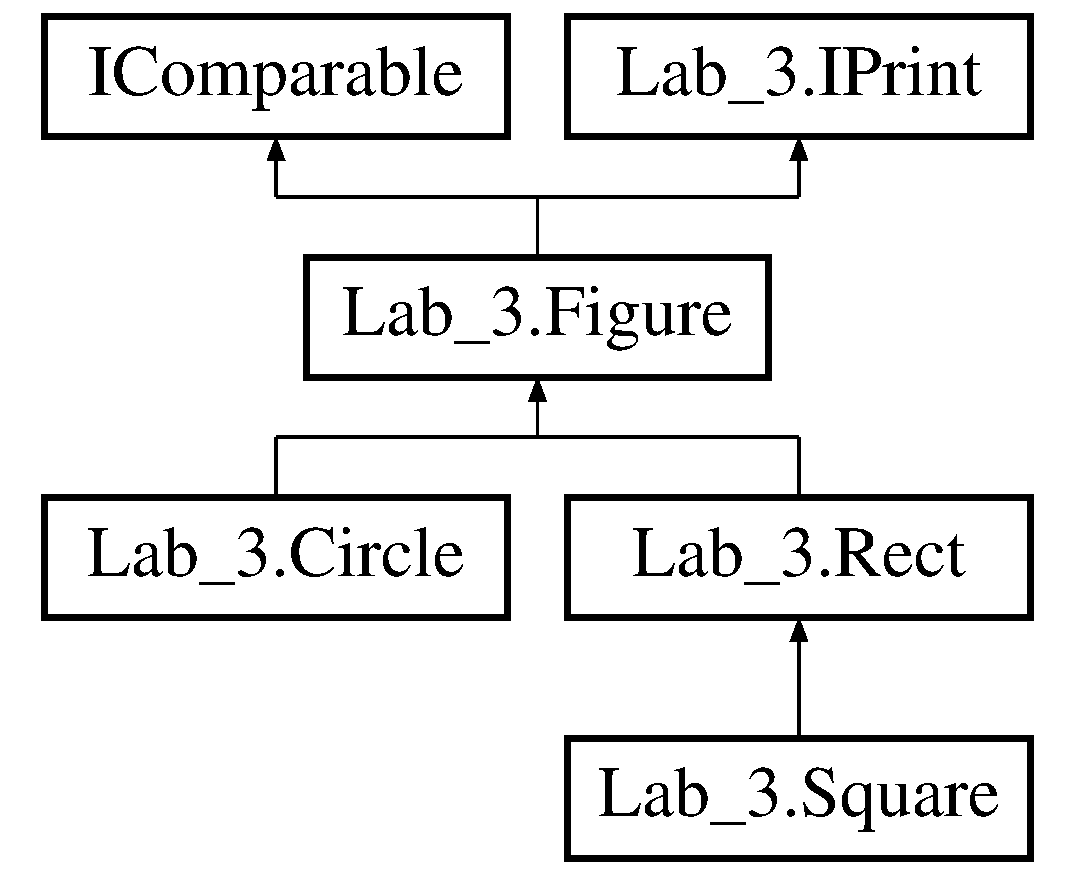
\includegraphics[height=4.000000cm]{class_lab__3_1_1_figure}
\end{center}
\end{figure}
\subsection*{Public Member Functions}
\begin{DoxyCompactItemize}
\item 
\mbox{\Hypertarget{class_lab__3_1_1_figure_a43f90db1a57fa8848845a5ec153568b8}\label{class_lab__3_1_1_figure_a43f90db1a57fa8848845a5ec153568b8}} 
virtual double {\bfseries square} ()
\item 
\mbox{\Hypertarget{class_lab__3_1_1_figure_a95235587aec0c4324f099727a76f3990}\label{class_lab__3_1_1_figure_a95235587aec0c4324f099727a76f3990}} 
int {\bfseries Compare\+To} (object obj)
\item 
\mbox{\Hypertarget{class_lab__3_1_1_figure_a71d86f8405dea8375268373a75337779}\label{class_lab__3_1_1_figure_a71d86f8405dea8375268373a75337779}} 
abstract void {\bfseries print} ()
\end{DoxyCompactItemize}


The documentation for this class was generated from the following file\+:\begin{DoxyCompactItemize}
\item 
Lab\+\_\+2\+\_\+\+Source.\+cs\end{DoxyCompactItemize}

\hypertarget{class_lab__3_1_1_figure_matrix_check_empty}{}\section{Lab\+\_\+3.\+Figure\+Matrix\+Check\+Empty Class Reference}
\label{class_lab__3_1_1_figure_matrix_check_empty}\index{Lab\+\_\+3.\+Figure\+Matrix\+Check\+Empty@{Lab\+\_\+3.\+Figure\+Matrix\+Check\+Empty}}
Inheritance diagram for Lab\+\_\+3.\+Figure\+Matrix\+Check\+Empty\+:\begin{figure}[H]
\begin{center}
\leavevmode
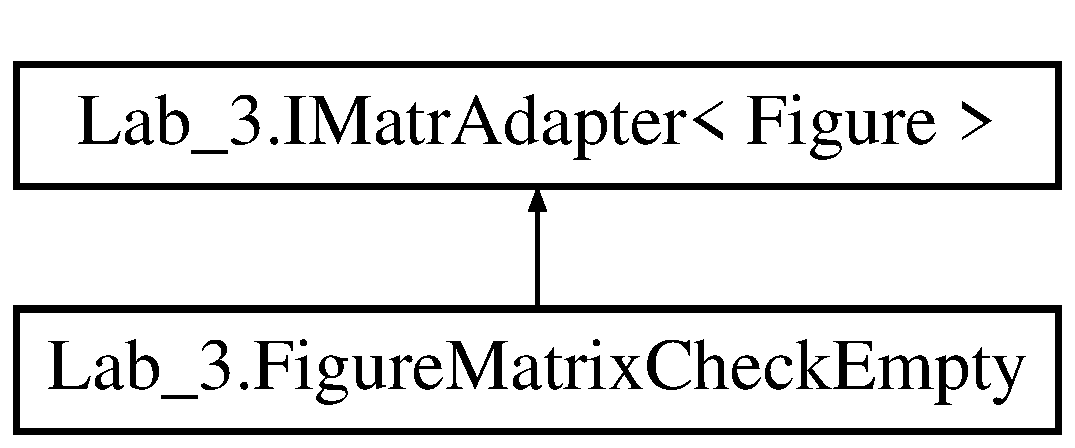
\includegraphics[height=2.000000cm]{class_lab__3_1_1_figure_matrix_check_empty}
\end{center}
\end{figure}
\subsection*{Additional Inherited Members}


The documentation for this class was generated from the following file\+:\begin{DoxyCompactItemize}
\item 
Lab\+\_\+3\+\_\+\+Source.\+cs\end{DoxyCompactItemize}

\hypertarget{interface_lab__3_1_1_i_matr_adapter}{}\section{Lab\+\_\+3.\+I\+Matr\+Adapter$<$ T $>$ Interface Template Reference}
\label{interface_lab__3_1_1_i_matr_adapter}\index{Lab\+\_\+3.\+I\+Matr\+Adapter$<$ T $>$@{Lab\+\_\+3.\+I\+Matr\+Adapter$<$ T $>$}}
\subsection*{Public Member Functions}
\begin{DoxyCompactItemize}
\item 
\mbox{\Hypertarget{interface_lab__3_1_1_i_matr_adapter_a9ebf65e14c3ab701aff51dce8182d47a}\label{interface_lab__3_1_1_i_matr_adapter_a9ebf65e14c3ab701aff51dce8182d47a}} 
T {\bfseries get\+Empty\+Element} ()
\item 
\mbox{\Hypertarget{interface_lab__3_1_1_i_matr_adapter_ab97cbc19e1eddfddf2224640f7dd8513}\label{interface_lab__3_1_1_i_matr_adapter_ab97cbc19e1eddfddf2224640f7dd8513}} 
bool {\bfseries check\+Empty\+Element} (T element)
\end{DoxyCompactItemize}


The documentation for this interface was generated from the following file\+:\begin{DoxyCompactItemize}
\item 
Lab\+\_\+3\+\_\+\+Source.\+cs\end{DoxyCompactItemize}

\hypertarget{interface_lab__3_1_1_i_print}{}\section{Lab\+\_\+3.\+I\+Print Interface Reference}
\label{interface_lab__3_1_1_i_print}\index{Lab\+\_\+3.\+I\+Print@{Lab\+\_\+3.\+I\+Print}}
Inheritance diagram for Lab\+\_\+3.\+I\+Print\+:\begin{figure}[H]
\begin{center}
\leavevmode
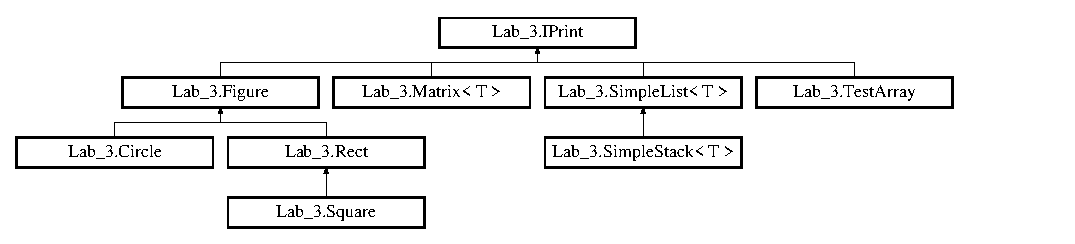
\includegraphics[height=2.835443cm]{interface_lab__3_1_1_i_print}
\end{center}
\end{figure}
\subsection*{Public Member Functions}
\begin{DoxyCompactItemize}
\item 
\mbox{\Hypertarget{interface_lab__3_1_1_i_print_a0584c14a36a3e38410d6c789cf0941e4}\label{interface_lab__3_1_1_i_print_a0584c14a36a3e38410d6c789cf0941e4}} 
void {\bfseries print} ()
\end{DoxyCompactItemize}


The documentation for this interface was generated from the following file\+:\begin{DoxyCompactItemize}
\item 
Lab\+\_\+2\+\_\+\+Source.\+cs\end{DoxyCompactItemize}

\hypertarget{class_lab__3_1_1_matrix}{}\section{Lab\+\_\+3.\+Matrix$<$ T $>$ Class Template Reference}
\label{class_lab__3_1_1_matrix}\index{Lab\+\_\+3.\+Matrix$<$ T $>$@{Lab\+\_\+3.\+Matrix$<$ T $>$}}
Inheritance diagram for Lab\+\_\+3.\+Matrix$<$ T $>$\+:\begin{figure}[H]
\begin{center}
\leavevmode
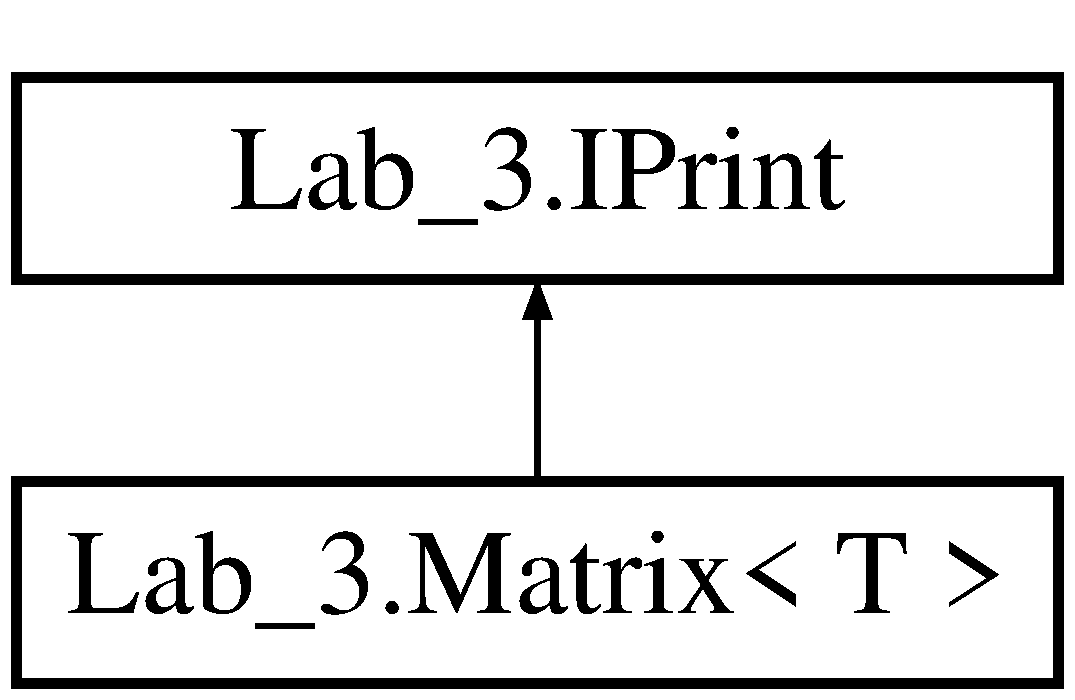
\includegraphics[height=2.000000cm]{class_lab__3_1_1_matrix}
\end{center}
\end{figure}
\subsection*{Public Member Functions}
\begin{DoxyCompactItemize}
\item 
\mbox{\Hypertarget{class_lab__3_1_1_matrix_ad27089ac3ced6a9be1b1a539c4bf648c}\label{class_lab__3_1_1_matrix_ad27089ac3ced6a9be1b1a539c4bf648c}} 
{\bfseries Matrix} (int \+\_\+xmax, int \+\_\+ymax, int \+\_\+zmax, \hyperlink{interface_lab__3_1_1_i_matr_adapter}{I\+Matr\+Adapter}$<$ T $>$ I\+M\+CE)
\item 
\mbox{\Hypertarget{class_lab__3_1_1_matrix_a57479fbdcf5cec14ba87e4262a31f2a4}\label{class_lab__3_1_1_matrix_a57479fbdcf5cec14ba87e4262a31f2a4}} 
override string {\bfseries To\+String} ()
\item 
\mbox{\Hypertarget{class_lab__3_1_1_matrix_a95b3ff17ea377e285ac5a994f8d417a5}\label{class_lab__3_1_1_matrix_a95b3ff17ea377e285ac5a994f8d417a5}} 
void {\bfseries print} ()
\end{DoxyCompactItemize}
\subsection*{Public Attributes}
\begin{DoxyCompactItemize}
\item 
\mbox{\Hypertarget{class_lab__3_1_1_matrix_a802a5a8fb9928f8e1a77c57890c5dd76}\label{class_lab__3_1_1_matrix_a802a5a8fb9928f8e1a77c57890c5dd76}} 
\hyperlink{interface_lab__3_1_1_i_matr_adapter}{I\+Matr\+Adapter}$<$ T $>$ {\bfseries Adap}
\end{DoxyCompactItemize}
\subsection*{Properties}
\begin{DoxyCompactItemize}
\item 
\mbox{\Hypertarget{class_lab__3_1_1_matrix_a6f092832b76bfe7d6e5d25f5e92d986d}\label{class_lab__3_1_1_matrix_a6f092832b76bfe7d6e5d25f5e92d986d}} 
T {\bfseries this\mbox{[}int x, int y, int z\mbox{]}}\hspace{0.3cm}{\ttfamily  \mbox{[}get, set\mbox{]}}
\end{DoxyCompactItemize}


The documentation for this class was generated from the following file\+:\begin{DoxyCompactItemize}
\item 
Lab\+\_\+3\+\_\+\+Source.\+cs\end{DoxyCompactItemize}

\hypertarget{class_lab__3_1_1_menu}{}\section{Lab\+\_\+3.\+Menu Class Reference}
\label{class_lab__3_1_1_menu}\index{Lab\+\_\+3.\+Menu@{Lab\+\_\+3.\+Menu}}
\subsection*{Public Member Functions}
\begin{DoxyCompactItemize}
\item 
\mbox{\Hypertarget{class_lab__3_1_1_menu_a99dafd028d14bc0ec37ebf4a59c66f76}\label{class_lab__3_1_1_menu_a99dafd028d14bc0ec37ebf4a59c66f76}} 
void {\bfseries run} ()
\end{DoxyCompactItemize}


The documentation for this class was generated from the following file\+:\begin{DoxyCompactItemize}
\item 
Lab\+\_\+3\+\_\+\+Source.\+cs\end{DoxyCompactItemize}

\hypertarget{class_lab__3_1_1_my_system}{}\section{Lab\+\_\+3.\+My\+System Class Reference}
\label{class_lab__3_1_1_my_system}\index{Lab\+\_\+3.\+My\+System@{Lab\+\_\+3.\+My\+System}}
\subsection*{Public Member Functions}
\begin{DoxyCompactItemize}
\item 
\mbox{\Hypertarget{class_lab__3_1_1_my_system_af5ddf1a60313be72cbc1455fd5a92d07}\label{class_lab__3_1_1_my_system_af5ddf1a60313be72cbc1455fd5a92d07}} 
void {\bfseries pause} ()
\item 
\mbox{\Hypertarget{class_lab__3_1_1_my_system_a35082095f042f3adfce8683da117ebb9}\label{class_lab__3_1_1_my_system_a35082095f042f3adfce8683da117ebb9}} 
void {\bfseries print\+Palka} (int l)
\item 
\mbox{\Hypertarget{class_lab__3_1_1_my_system_af9f46e3d19237b659c7e51453fb57323}\label{class_lab__3_1_1_my_system_af9f46e3d19237b659c7e51453fb57323}} 
\hyperlink{class_lab__3_1_1_figure}{Figure} {\bfseries Gener\+Figure} (int param, Random rand)
\end{DoxyCompactItemize}


The documentation for this class was generated from the following file\+:\begin{DoxyCompactItemize}
\item 
My\+System.\+cs\end{DoxyCompactItemize}

\hypertarget{class_lab__3_1_1_program}{}\section{Lab\+\_\+3.\+Program Class Reference}
\label{class_lab__3_1_1_program}\index{Lab\+\_\+3.\+Program@{Lab\+\_\+3.\+Program}}


The documentation for this class was generated from the following file\+:\begin{DoxyCompactItemize}
\item 
Program.\+cs\end{DoxyCompactItemize}

\hypertarget{class_lab__3_1_1_rect}{}\section{Lab\+\_\+3.\+Rect Class Reference}
\label{class_lab__3_1_1_rect}\index{Lab\+\_\+3.\+Rect@{Lab\+\_\+3.\+Rect}}
Inheritance diagram for Lab\+\_\+3.\+Rect\+:\begin{figure}[H]
\begin{center}
\leavevmode
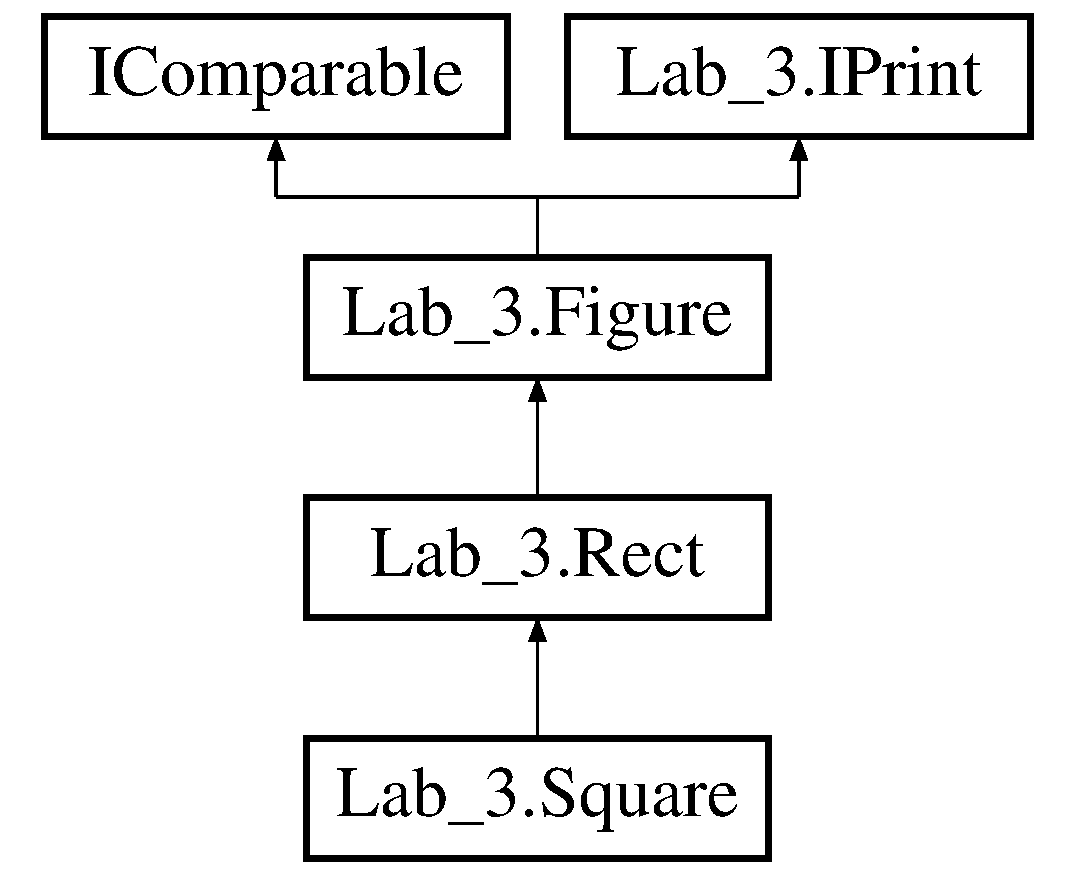
\includegraphics[height=4.000000cm]{class_lab__3_1_1_rect}
\end{center}
\end{figure}
\subsection*{Public Member Functions}
\begin{DoxyCompactItemize}
\item 
\mbox{\Hypertarget{class_lab__3_1_1_rect_a285ef8c42d2a06f04f09ef6e7b9c22f9}\label{class_lab__3_1_1_rect_a285ef8c42d2a06f04f09ef6e7b9c22f9}} 
{\bfseries Rect} (double a1, double b1)
\item 
\mbox{\Hypertarget{class_lab__3_1_1_rect_addfcdb058f6a7440f43dbcf30fde6104}\label{class_lab__3_1_1_rect_addfcdb058f6a7440f43dbcf30fde6104}} 
override string {\bfseries To\+String} ()
\item 
\mbox{\Hypertarget{class_lab__3_1_1_rect_a79f99909e2828a192aee47e2f85cb3fc}\label{class_lab__3_1_1_rect_a79f99909e2828a192aee47e2f85cb3fc}} 
override double {\bfseries square} ()
\item 
\mbox{\Hypertarget{class_lab__3_1_1_rect_ac7cc4646c13003bd1b373fd2177ac84d}\label{class_lab__3_1_1_rect_ac7cc4646c13003bd1b373fd2177ac84d}} 
override void {\bfseries print} ()
\end{DoxyCompactItemize}
\subsection*{Properties}
\begin{DoxyCompactItemize}
\item 
\mbox{\Hypertarget{class_lab__3_1_1_rect_aa7abab101cbf1b8dec773453d51f5377}\label{class_lab__3_1_1_rect_aa7abab101cbf1b8dec773453d51f5377}} 
virtual double {\bfseries A}\hspace{0.3cm}{\ttfamily  \mbox{[}get, set\mbox{]}}
\item 
\mbox{\Hypertarget{class_lab__3_1_1_rect_a1c568dcd9446e9e36736d38e691bd23f}\label{class_lab__3_1_1_rect_a1c568dcd9446e9e36736d38e691bd23f}} 
virtual double {\bfseries B}\hspace{0.3cm}{\ttfamily  \mbox{[}get, set\mbox{]}}
\end{DoxyCompactItemize}


The documentation for this class was generated from the following file\+:\begin{DoxyCompactItemize}
\item 
Lab\+\_\+2\+\_\+\+Source.\+cs\end{DoxyCompactItemize}

\hypertarget{class_lab__3_1_1_simple_list}{}\section{Lab\+\_\+3.\+Simple\+List$<$ T $>$ Class Template Reference}
\label{class_lab__3_1_1_simple_list}\index{Lab\+\_\+3.\+Simple\+List$<$ T $>$@{Lab\+\_\+3.\+Simple\+List$<$ T $>$}}
Inheritance diagram for Lab\+\_\+3.\+Simple\+List$<$ T $>$\+:\begin{figure}[H]
\begin{center}
\leavevmode
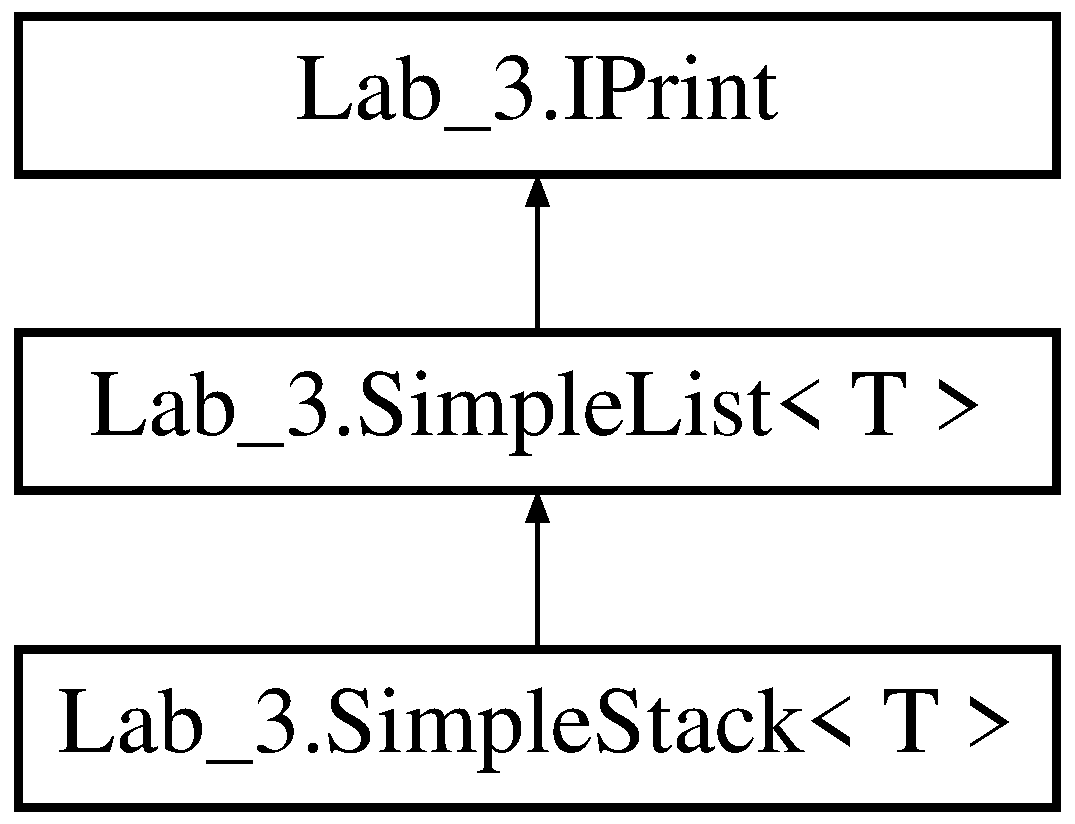
\includegraphics[height=3.000000cm]{class_lab__3_1_1_simple_list}
\end{center}
\end{figure}
\subsection*{Public Member Functions}
\begin{DoxyCompactItemize}
\item 
\mbox{\Hypertarget{class_lab__3_1_1_simple_list_a9bd28dd4f80bf25e7c05d85be8f913f3}\label{class_lab__3_1_1_simple_list_a9bd28dd4f80bf25e7c05d85be8f913f3}} 
void {\bfseries Add} (T element)
\item 
\mbox{\Hypertarget{class_lab__3_1_1_simple_list_a81f906eafcb867d5d10ca323456dbf70}\label{class_lab__3_1_1_simple_list_a81f906eafcb867d5d10ca323456dbf70}} 
\hyperlink{class_lab__3_1_1_simple_list_item}{Simple\+List\+Item}$<$ T $>$ {\bfseries get\+Item} (int number)
\item 
\mbox{\Hypertarget{class_lab__3_1_1_simple_list_ac3bdb6cf211c6def760744914c89bac0}\label{class_lab__3_1_1_simple_list_ac3bdb6cf211c6def760744914c89bac0}} 
T {\bfseries Get} (int number)
\item 
\mbox{\Hypertarget{class_lab__3_1_1_simple_list_a06c6221695fe05b4e55d1d326bd34c68}\label{class_lab__3_1_1_simple_list_a06c6221695fe05b4e55d1d326bd34c68}} 
override string {\bfseries To\+String} ()
\item 
\mbox{\Hypertarget{class_lab__3_1_1_simple_list_add4d78c448d7b3a8cb290b2d1fac89fa}\label{class_lab__3_1_1_simple_list_add4d78c448d7b3a8cb290b2d1fac89fa}} 
void {\bfseries print} ()
\end{DoxyCompactItemize}
\subsection*{Protected Attributes}
\begin{DoxyCompactItemize}
\item 
\mbox{\Hypertarget{class_lab__3_1_1_simple_list_a8c098afd105a16fcd767afbc089718ef}\label{class_lab__3_1_1_simple_list_a8c098afd105a16fcd767afbc089718ef}} 
\hyperlink{class_lab__3_1_1_simple_list_item}{Simple\+List\+Item}$<$ T $>$ {\bfseries first}
\item 
\mbox{\Hypertarget{class_lab__3_1_1_simple_list_abd536e79607687158336cd9a29be41dd}\label{class_lab__3_1_1_simple_list_abd536e79607687158336cd9a29be41dd}} 
\hyperlink{class_lab__3_1_1_simple_list_item}{Simple\+List\+Item}$<$ T $>$ {\bfseries last}
\end{DoxyCompactItemize}
\subsection*{Properties}
\begin{DoxyCompactItemize}
\item 
\mbox{\Hypertarget{class_lab__3_1_1_simple_list_a988b7dc1b39feced3a83dcc77fba7da9}\label{class_lab__3_1_1_simple_list_a988b7dc1b39feced3a83dcc77fba7da9}} 
int {\bfseries count}\hspace{0.3cm}{\ttfamily  \mbox{[}get, protected set\mbox{]}}
\end{DoxyCompactItemize}


The documentation for this class was generated from the following file\+:\begin{DoxyCompactItemize}
\item 
Lab\+\_\+3\+\_\+\+Source.\+cs\end{DoxyCompactItemize}

\hypertarget{class_lab__3_1_1_simple_list_item}{}\section{Lab\+\_\+3.\+Simple\+List\+Item$<$ T $>$ Class Template Reference}
\label{class_lab__3_1_1_simple_list_item}\index{Lab\+\_\+3.\+Simple\+List\+Item$<$ T $>$@{Lab\+\_\+3.\+Simple\+List\+Item$<$ T $>$}}
\subsection*{Public Member Functions}
\begin{DoxyCompactItemize}
\item 
\mbox{\Hypertarget{class_lab__3_1_1_simple_list_item_a2f000338a7cb0d59db8f97d3d0863da4}\label{class_lab__3_1_1_simple_list_item_a2f000338a7cb0d59db8f97d3d0863da4}} 
{\bfseries Simple\+List\+Item} (T param)
\end{DoxyCompactItemize}
\subsection*{Properties}
\begin{DoxyCompactItemize}
\item 
\mbox{\Hypertarget{class_lab__3_1_1_simple_list_item_afdee6166185faa715750d67cd1142787}\label{class_lab__3_1_1_simple_list_item_afdee6166185faa715750d67cd1142787}} 
T {\bfseries data}\hspace{0.3cm}{\ttfamily  \mbox{[}get, set\mbox{]}}
\item 
\mbox{\Hypertarget{class_lab__3_1_1_simple_list_item_a06c3e2383cacf8d7b0d5e619c90caea2}\label{class_lab__3_1_1_simple_list_item_a06c3e2383cacf8d7b0d5e619c90caea2}} 
\hyperlink{class_lab__3_1_1_simple_list_item}{Simple\+List\+Item}$<$ T $>$ {\bfseries next}\hspace{0.3cm}{\ttfamily  \mbox{[}get, set\mbox{]}}
\end{DoxyCompactItemize}


The documentation for this class was generated from the following file\+:\begin{DoxyCompactItemize}
\item 
Lab\+\_\+3\+\_\+\+Source.\+cs\end{DoxyCompactItemize}

\hypertarget{class_lab__3_1_1_simple_stack}{}\section{Lab\+\_\+3.\+Simple\+Stack$<$ T $>$ Class Template Reference}
\label{class_lab__3_1_1_simple_stack}\index{Lab\+\_\+3.\+Simple\+Stack$<$ T $>$@{Lab\+\_\+3.\+Simple\+Stack$<$ T $>$}}
Inheritance diagram for Lab\+\_\+3.\+Simple\+Stack$<$ T $>$\+:\begin{figure}[H]
\begin{center}
\leavevmode
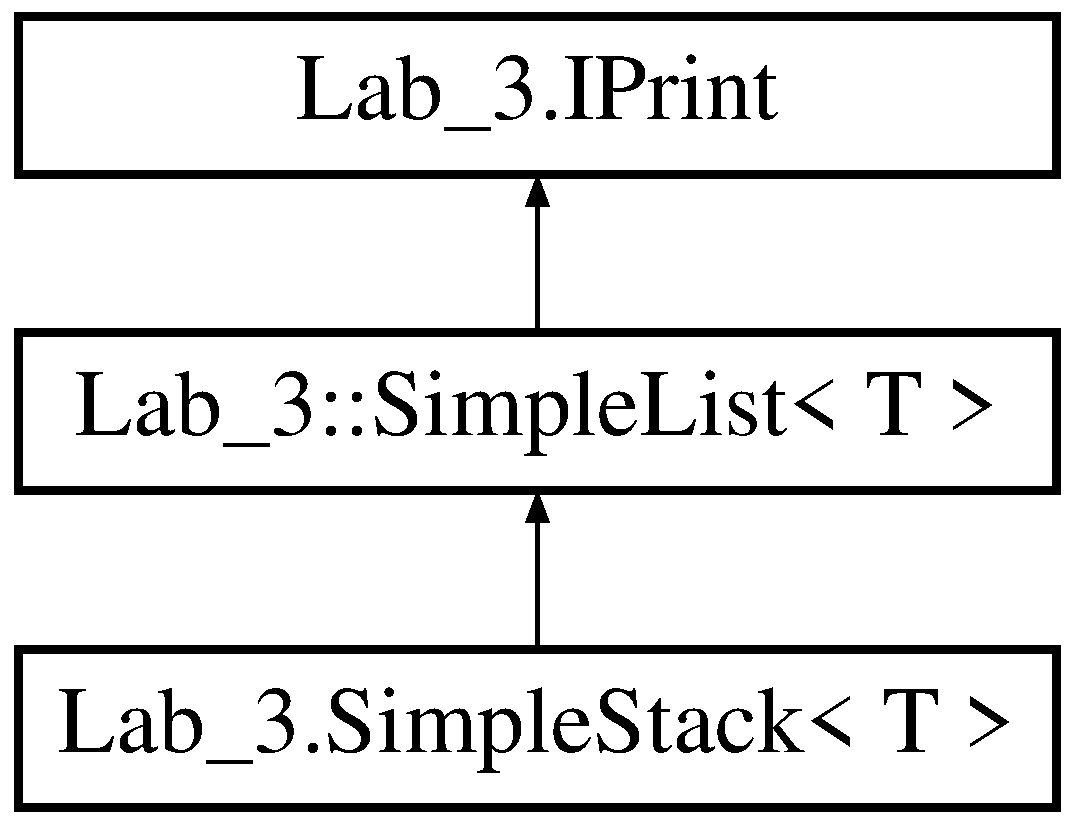
\includegraphics[height=3.000000cm]{class_lab__3_1_1_simple_stack}
\end{center}
\end{figure}
\subsection*{Public Member Functions}
\begin{DoxyCompactItemize}
\item 
\mbox{\Hypertarget{class_lab__3_1_1_simple_stack_a2d3f3ff8776f484420b01e8812a07ae8}\label{class_lab__3_1_1_simple_stack_a2d3f3ff8776f484420b01e8812a07ae8}} 
\hyperlink{class_lab__3_1_1_simple_list_item}{Simple\+List\+Item}$<$ T $>$ {\bfseries Pop} (int i)
\item 
\mbox{\Hypertarget{class_lab__3_1_1_simple_stack_a4315fe36c3b6ae612278243b5d5ba7ec}\label{class_lab__3_1_1_simple_stack_a4315fe36c3b6ae612278243b5d5ba7ec}} 
void {\bfseries Push} (T element)
\end{DoxyCompactItemize}
\subsection*{Additional Inherited Members}


The documentation for this class was generated from the following file\+:\begin{DoxyCompactItemize}
\item 
Lab\+\_\+3\+\_\+\+Source.\+cs\end{DoxyCompactItemize}

\hypertarget{class_lab__3_1_1_square}{}\section{Lab\+\_\+3.\+Square Class Reference}
\label{class_lab__3_1_1_square}\index{Lab\+\_\+3.\+Square@{Lab\+\_\+3.\+Square}}
Inheritance diagram for Lab\+\_\+3.\+Square\+:\begin{figure}[H]
\begin{center}
\leavevmode
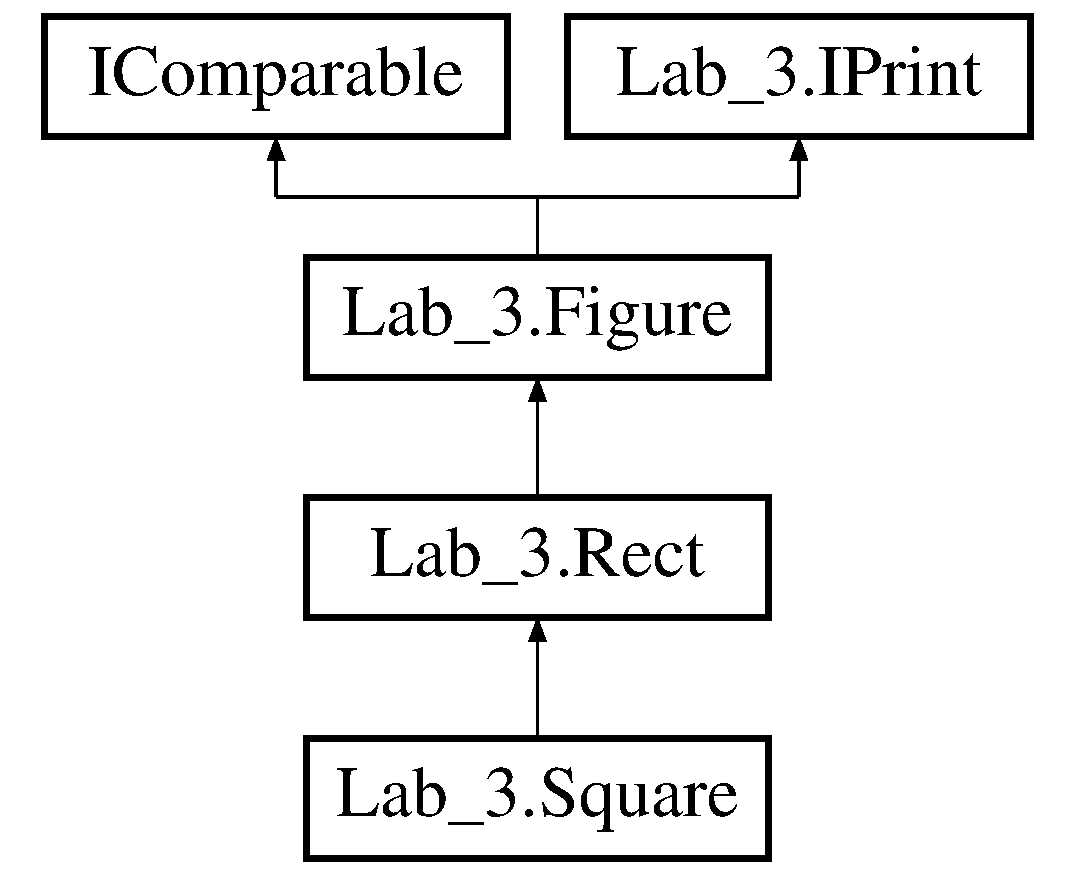
\includegraphics[height=4.000000cm]{class_lab__3_1_1_square}
\end{center}
\end{figure}
\subsection*{Public Member Functions}
\begin{DoxyCompactItemize}
\item 
\mbox{\Hypertarget{class_lab__3_1_1_square_a1326003724f6f8dee493a8f98c8e797b}\label{class_lab__3_1_1_square_a1326003724f6f8dee493a8f98c8e797b}} 
override string {\bfseries To\+String} ()
\item 
\mbox{\Hypertarget{class_lab__3_1_1_square_a9fefca730022f798f20b958f1a62b3d7}\label{class_lab__3_1_1_square_a9fefca730022f798f20b958f1a62b3d7}} 
{\bfseries Square} (double a1)
\end{DoxyCompactItemize}
\subsection*{Additional Inherited Members}


The documentation for this class was generated from the following file\+:\begin{DoxyCompactItemize}
\item 
Lab\+\_\+2\+\_\+\+Source.\+cs\end{DoxyCompactItemize}

\hypertarget{class_lab__3_1_1_test_array}{}\section{Lab\+\_\+3.\+Test\+Array Class Reference}
\label{class_lab__3_1_1_test_array}\index{Lab\+\_\+3.\+Test\+Array@{Lab\+\_\+3.\+Test\+Array}}
Inheritance diagram for Lab\+\_\+3.\+Test\+Array\+:\begin{figure}[H]
\begin{center}
\leavevmode
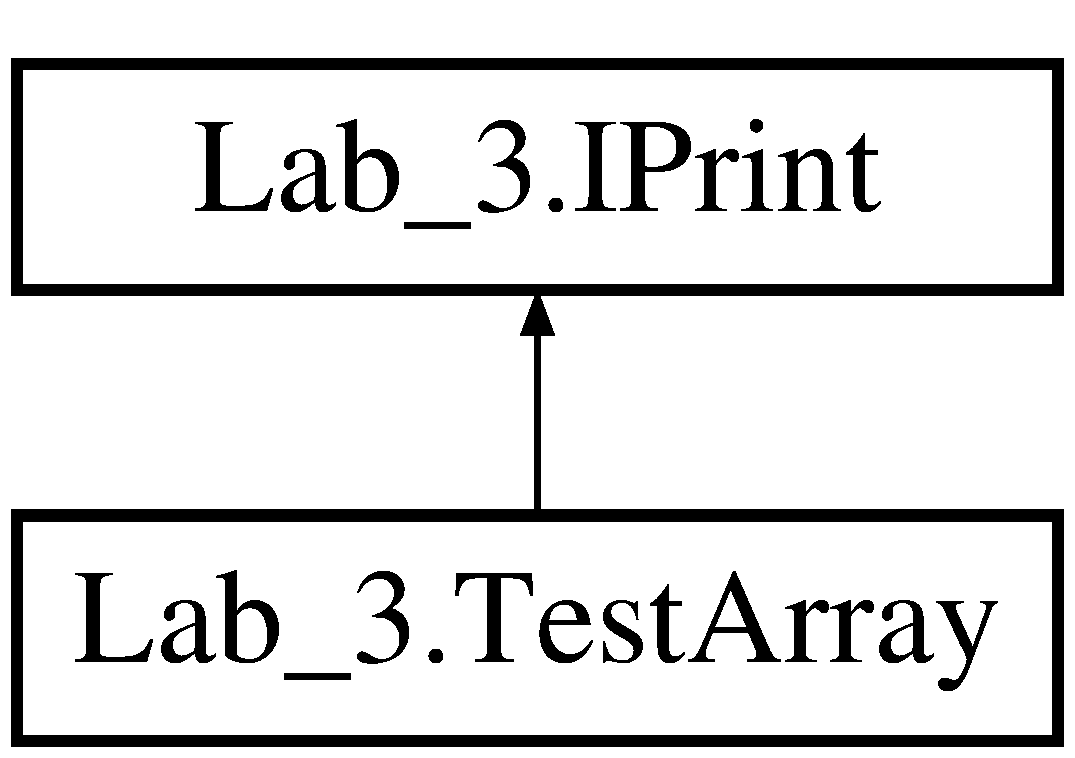
\includegraphics[height=2.000000cm]{class_lab__3_1_1_test_array}
\end{center}
\end{figure}
\subsection*{Public Member Functions}
\begin{DoxyCompactItemize}
\item 
\mbox{\Hypertarget{class_lab__3_1_1_test_array_a6e4384a2b48ea601c8cc3fcbfefbdb15}\label{class_lab__3_1_1_test_array_a6e4384a2b48ea601c8cc3fcbfefbdb15}} 
void {\bfseries Gener} (int rmax, int times)
\item 
\mbox{\Hypertarget{class_lab__3_1_1_test_array_ab3fec5626a043e0d31e40634698e3c24}\label{class_lab__3_1_1_test_array_ab3fec5626a043e0d31e40634698e3c24}} 
void {\bfseries print} ()
\item 
\mbox{\Hypertarget{class_lab__3_1_1_test_array_a10bf97ffef85d7548db03396342980ea}\label{class_lab__3_1_1_test_array_a10bf97ffef85d7548db03396342980ea}} 
void {\bfseries Sort} ()
\end{DoxyCompactItemize}


The documentation for this class was generated from the following file\+:\begin{DoxyCompactItemize}
\item 
Lab\+\_\+3\+\_\+\+Source.\+cs\end{DoxyCompactItemize}

%--- End generated contents ---

% Index
\backmatter
\newpage
\phantomsection
\clearemptydoublepage
\addcontentsline{toc}{chapter}{Index}
\printindex

\end{document}
